\chapter{Ironic镜像制作}
\section{安装必要软件}
\begin{code-block}{bash}
yum install diskimage-builder libguestfs-tools libguestfs-tools-c libguestfs-xfs libvirt -y
systemctl enable libvirtd
systemctl start libvirtd
\end{code-block}

{\color{red}请一定注意,要求diskimage-builder 的版本必须<=1.14.1-1,否则可能出现问题。}

如果是制作windows的镜像,请在windows10操作系统上做如下操作:
\begin{itemize}
  \item 开启hyper-v虚拟化
  \item 安装adk:https://developer.microsoft.com/en-us/windows/hardware/windows-assessment-deployment-kit
  \item 开启powershell的脚本执行策略:Set-ExecutionPolicy -ExecutionPolicy BYPASS
  \item 下载镜像制作工具:git clone https://github.com/luoyancn/windows-images-tools-for-ironic
\end{itemize}

\section{制作centos6.x镜像}
\subsection{创建centos6x / redhat6x的虚拟机}
虚拟机的安装和普通的虚拟机安装和操作没有太大的区别,但是,磁盘文件必须是qcow2的格式,另外磁盘分区部分需要格外注意,
{\color{red}绝对不能使用lvm的磁盘分区,必须使用标准分区。}

\subsection{修改centos6x / redhat6x虚拟机操作系统内部参数}
\begin{code-block}{bash}
# 关闭selinux
sed -i 's/=enforcing/=disabled/g' /etc/selinux/config
# 关闭iptables
service iptables stop
chkconfig iptables off
# 修改网卡rule文件
echo > /etc/udev/rules.d/70-persistent-net.rules
chattr +i /etc/udev/rules.d/70-persistent-net.rules
# 修改网卡配置文件
cat >/etc/sysconfig/network-scripts/ifcfg-eth0<<EOF
DEVICE=eth0
TYPE=Ethernet
ONBOOT=yes
NM_CONTROLLED=no
BOOTPROTO=dhcp
EOF
# 安装centos6的epel源
yum install https://mirrors.ustc.edu.cn/epel/6/x86_64/epel-release-6-8.noarch.rpm -y
\end{code-block}

如果是redhat6x的虚拟机,还需要对yum源做一些列的操作,添加额外的repo,来支持之后的一些列的操作
\begin{code-block}{bash}
rm -rf /etc/yum.repos.d/*.repo
sed -i 's/plugins=1/plugins=0/g' /etc/yum.conf
cat > /etc/yum.repos.d/cern-6.repo<<EOF
[cern-extra]
name=cern-extra
baseurl=http://linuxsoft.cern.ch/cern/slc6X/extras/x86_64/RPMS/
enabled=1
gpgcheck=0
[cern-update]
name=cern-update
baseurl=http://linuxsoft.cern.ch/cern/slc6X/updates/x86_64/RPMS/
enabled=1
gpgcheck=0
[cern-slc]
name=cern-slc
baseurl=http://linuxsoft.cern.ch/cern/slc6X/x86_64/SLC/
enabled=1
gpgcheck=0
EOF
\end{code-block}

\subsection{检查参数设置以及安装必要的软件}
\begin{code-block}{bash}
yum install cloud-utils-growpart python-argparse -y
\end{code-block}

以上步骤结束之后,关闭虚拟机,保留虚拟机的磁盘文件备用。

\subsection{转换虚拟机镜像文件为物理机可以使用的镜像}

设置环境变量
\begin{code-block}{bash}
export DIB_DEV_USER_PASSWORD="cloud"
export DIB_DEV_USER_USERNAME="cloud"
export DIB_DEV_USER_PWDLESS_SUDO="yes"
export DIB_LOCAL_IMAGE=/opt/centos6
\end{code-block}

转换镜像
\begin{code-block}{bash}
disk-image-create centos devuser baremetal enable-serial-console cloud-init dhcp-all-interfaces vm -o centos6 -t qcow2
\end{code-block}

修改和校验镜像
\begin{code-block}{bash}
# 打开镜像文件
guestmount -a /opt/centos6.qcow2 -m /dev/sda1 /mnt/
# 校验selinux是否关闭
cat /mnt/etc/selinux/config # 看SELINUX=disabled
# 校验必须的命令是否存在,# 正常的输出应该为/mnt/usr/bin/growpart: POSIX shell script, ASCII text executable
file /mnt/usr/bin/growpart
# 修改cloud-init的配置文件
vi /mnt/etc/cloud/cloud.cfg
# 具体内容请参照 后续cloud-init的具体内容
# 追加cloud.cfg的内容
runcmd:
 - reboot
# 添加网卡配置文件
cat >/mnt/etc/sysconfig/network-scripts/ifcfg-eth0<<EOF
DEVICE=eth0
TYPE=Ethernet
ONBOOT=yes
NM_CONTROLLED=no
BOOTPROTO=dhcp
EOF

# 确定没有需要修改和校验的地方之后,关闭镜像文件
guestunmount /mnt
\end{code-block}

经过以上的操作之后,镜像制作完毕,可以用于部署物理机了。

\section{制作centos7.x镜像}
\subsection{创建centos7x / redhat7x的虚拟机}
虚拟机的安装和普通的虚拟机安装和操作没有太大的区别,但是,磁盘文件必须是qcow2的格式,另外磁盘分区部分需要格外注意,
{\color{red}绝对不能使用lvm的磁盘分区,必须使用标准分区。}

\subsection{修改centos6x / redhat6x虚拟机操作系统内部参数}
\begin{code-block}{bash}
# 关闭selinux
sed -i 's/=enforcing/=disabled/g' /etc/selinux/config
# 卸载NetworkManager
yum erase NetworkManager -y
# 关闭iptables和NetworkManager
systemctl disable firewalld
systemctl enable network
# 修改网卡配置文件
cat >/etc/sysconfig/network-scripts/ifcfg-ens3<<EOF
TYPE=Ethernet
BOOTPROTO=dhcp
DEFROUTE=yes
PEERDNS=yes
PEERROUTES=yes
IPV4_FAILURE_FATAL=no
IPV6INIT=no
NAME=ens3
DEVICE=ens3
ONBOOT=yes
EOF
\end{code-block}

如果是redhat7x的虚拟机,还需要对yum源做一些列的操作,添加额外的repo,来支持之后的一些列的操作
\begin{code-block}{bash}
rm -rf /etc/yum.repos.d/*.repo
sed -i 's/plugins=1/plugins=0/g' /etc/yum.conf
cat > /etc/yum.repos.d/cern-7.repo<<EOF
[cern-os]
name=cern-os
baseurl=http://linuxsoft.cern.ch/cern/centos/7/os/x86_64/
gpgcheck=1
enabled=1
protect=1
priority=5
gpgkey=http://linuxsoft.cern.ch/cern/centos/7/os/x86_64/RPM-GPG-KEY-CentOS-7
[cern-centosplus]
name=cern-centosplus
baseurl=http://linuxsoft.cern.ch/cern/centos/7/centosplus/x86_64/
gpgcheck=0
enabled=1
protect=1
priority=5
gpgkey=http://linuxsoft.cern.ch/cern/centos/7/os/x86_64/RPM-GPG-KEY-CentOS-7
[cern-cern]
name=cern-cern
baseurl=http://linuxsoft.cern.ch/cern/centos/7/cern/x86_64/
gpgcheck=0
enabled=1
protect=1
priority=5
gpgkey=http://linuxsoft.cern.ch/cern/centos/7/os/x86_64/RPM-GPG-KEY-cern
[cern-extra]
name=cern-extra
baseurl=http://linuxsoft.cern.ch/cern/centos/7/extras/x86_64/
gpgcheck=0
enabled=1
protect=1
priority=5
gpgkey=http://linuxsoft.cern.ch/cern/centos/7/os/x86_64/RPM-GPG-KEY-cern
[cern-update]
name=cern-update
baseurl=http://linuxsoft.cern.ch/cern/centos/7/updates/x86_64/
gpgcheck=0
enabled=1
protect=1
priority=5
gpgkey=http://linuxsoft.cern.ch/cern/centos/7/os/x86_64/RPM-GPG-KEY-cern
[cern-cr]
name=cern-cr
baseurl=http://linuxsoft.cern.ch/cern/centos/7/cr/x86_64/
gpgcheck=0
enabled=1
protect=1
priority=5
gpgkey=http://linuxsoft.cern.ch/cern/centos/7/os/x86_64/RPM-GPG-KEY-cern
[cern-rt]
name=cern-rt
baseurl=http://linuxsoft.cern.ch/cern/centos/7/rt/x86_64/
gpgcheck=0
enabled=1
protect=1
priority=5
gpgkey=http://linuxsoft.cern.ch/cern/centos/7/os/x86_64/RPM-GPG-KEY-cern
[cern-rhcommon]
name=cern-rhcommon
baseurl=http://linuxsoft.cern.ch/cern/centos/7/rhcommon/x86_64/
gpgcheck=0
enabled=1
protect=1
priority=5
gpgkey=http://linuxsoft.cern.ch/cern/centos/7/os/x86_64/RPM-GPG-KEY-cern
[cern-epel]
name=cern-epel
baseurl=http://linuxsoft.cern.ch/epel/7/x86_64/
gpgcheck=0
enabled=1
protect=1
priority=5
gpgkey=http://linuxsoft.cern.ch/epel/RPM-GPG-KEY-EPEL-7
EOF
\end{code-block}

重启虚拟机。

\subsection{检查参数设置以及安装必要的软件}
\begin{code-block}{bash}
yum install cloud-utils-growpart -y
\end{code-block}

关闭虚拟机,保留虚拟机的磁盘文件。

\subsection{转换虚拟机镜像文件为物理机可以使用的镜像}

设置环境变量
\begin{code-block}{bash}
export DIB_DEV_USER_PASSWORD="cloud"
export DIB_DEV_USER_USERNAME="cloud"
export DIB_DEV_USER_PWDLESS_SUDO="yes"
export DIB_LOCAL_IMAGE=/opt/centos7
export FS_TYPE="xfs"
\end{code-block}

转换镜像
\begin{code-block}{bash}
disk-image-create centos7 devuser baremetal enable-serial-console cloud-init dhcp-all-interfaces vm \
        -o centos7-disk-image-builder -t qcow2
\end{code-block}

修改和校验镜像
\begin{code-block}{bash}
# 打开镜像文件
guestmount -a /opt/centos7-disk-image-builder.qcow2 -m /dev/sda1 /mnt/
# 校验selinux是否关闭
cat /mnt/etc/selinux/config # 看SELINUX=disabled
# 校验必须的命令是否存在,# 正常的输出应该为/mnt/usr/bin/growpart: POSIX shell script, ASCII text executable
file /mnt/usr/bin/growpart
# 修改cloud-init的配置文件
vi /mnt/etc/cloud/cloud.cfg
# 具体内容请参照 后续cloud-init的具体内容
# 确定没有需要修改和校验的地方之后,关闭镜像文件
guestunmount /mnt
\end{code-block}

经过以上操作之后,修改之后的镜像就可以提供给ironic部署物理机所使用了。

\section{制作ubuntu镜像}
制作ubuntu的ironic镜像必须能够连接公网。不仅是ubuntu,只要是制作linux的镜像,一律都需要连接公网
ubuntu的镜像制作相对简单。

设置环境变量
\begin{code-block}{bash}
export DIB_DEV_USER_PASSWORD="cloud"
export DIB_DEV_USER_USERNAME="cloud"
export DIB_DEV_USER_PWDLESS_SUDO="yes"
export DIB_RELEASE=xenial
\end{code-block}

需要注意的是DIB\_RELEASE表示的是ubuntu的版本代号,而不是版本号。关于版本代号和版本号之间的对应关系,请查询ubuntu官方网站。下方仅列出常用的ubuntu的版本号与代号之间的关系。
\begin{center}
  \rowcolors{2}{green!80!yellow!50}{green!70!yellow!40}
  %\begin{tabularx}{\textwidth}{|l|l|}
  \begin{tabularx}{0.2\textwidth}{|l|l|}
  \hline
  版本号& 版本代号\\ \hline
  14.04 & trusty \\
  16.04 & xenial \\
  \hline
  \end{tabularx}
  \label{tab:Binary files}
\end{center}

制作ubuntu镜像
\begin{code-block}{bash}
disk-image-create ubuntu devuser baremetal enable-serial-console cloud-init dhcp-all-interfaces vm \
        -o ubuntu14.04-xenial-disk-image-builder -t qcow2
\end{code-block}

修改ubuntu镜像
\begin{code-block}{bash}
# 打开镜像文件
guestmount -a /opt/ubuntu14.04-trusty-disk-image-builder.qcow2 -m /dev/sda1 /mnt/
# 修改sshd配置,允许远程登录
sed -i 's/PermitRootLogin without-password/PermitRootLogin yes/g' /mnt/etc/ssh/sshd_config
# 生成ssh所需要的文件
ssh-keygen  -t rsa -P "" -f  /mnt/etc/ssh/ssh_host_rsa_key
ssh-keygen  -t dsa -P "" -f  /mnt/etc/ssh/ssh_host_dsa_key
vi /mnt/etc/cloud/cloud.cfg
# 具体内容请参照 http://wiki.corp.awcloud.com/pages/viewpage.action?pageId=57704707
guestunmount /mnt
\end{code-block}

经过以上操作之后,修改之后的镜像就可以提供给ironic部署物理机所使用了

\section{制作windows 2012 R2 64/ 2016 64镜像}
特别注意,windows 2012 R2 64/ 2016 64的ironic镜像必须在windows物理机上制作,其他环境不可用
创建需要的目录, E:/hyper-v提取install.wim文件以及准备驱动文件将install.wim放到E:/hyper-v
\begin{figure}[H]
  \centering
  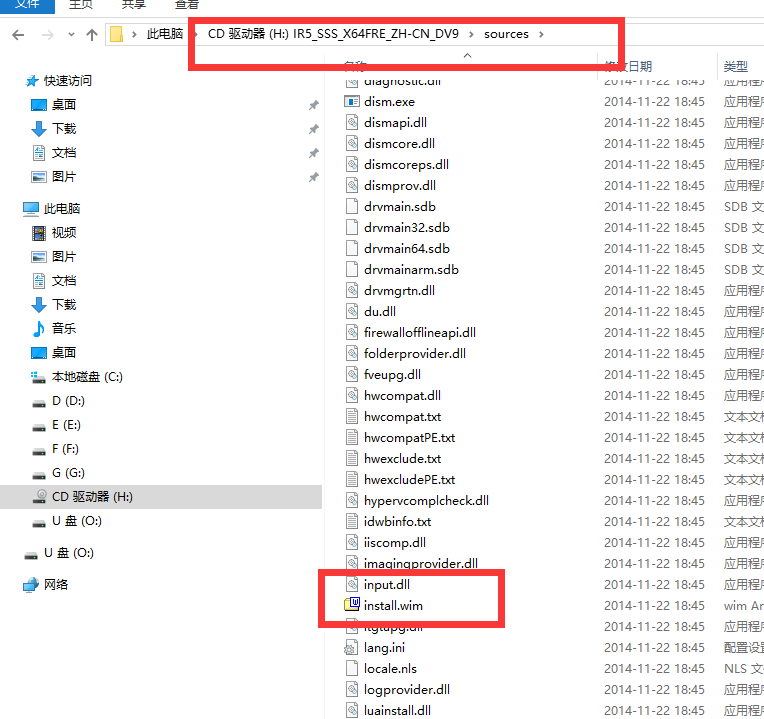
\includegraphics[scale=0.4]{installwim.png}
  \caption{install.wim文件}
  \label{fig:installwim}
\end{figure}

把驱动文件放到E:/hyper-v/2012\_r2\_64\_drivers。必驱动文件有如下的要求:须和目标硬件匹配/兼容, 必须是inf格式的驱动文件,不能是exe和msi的驱动。
目前可用的驱动可以在镜像转换工具当中找到。

改镜像制作工具代码, create-windows-online-cloud-image.ps1修改如下
\begin{figure}[H]
  \centering
  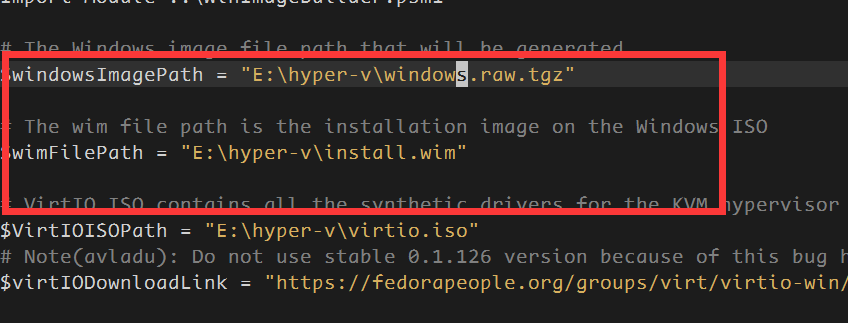
\includegraphics[width=\linewidth]{ps1.png}
  \caption{ps1}
  \label{fig:ps1}
\end{figure}
\begin{figure}[H]
  \centering
  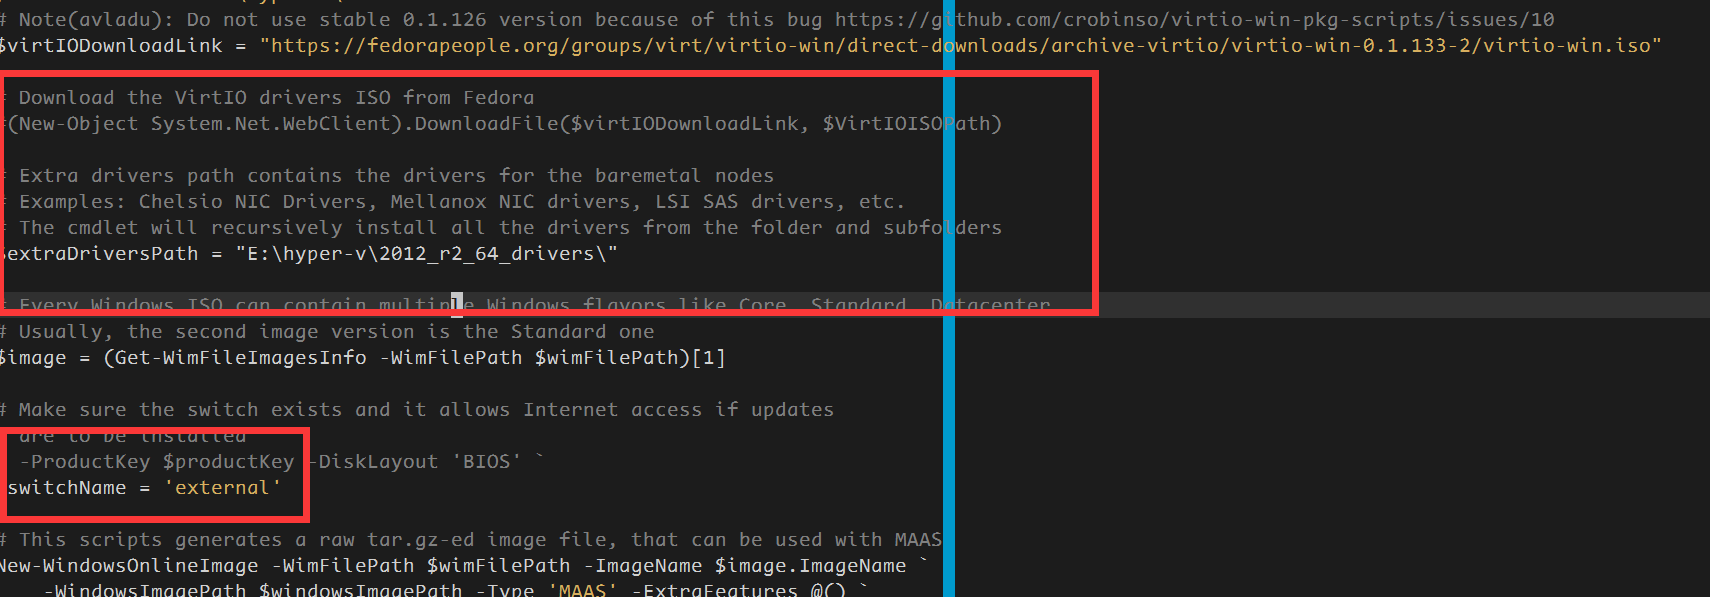
\includegraphics[width=\linewidth]{ps2.png}
  \caption{ps2}
  \label{fig:ps2}
\end{figure}
\begin{figure}[H]
  \centering
  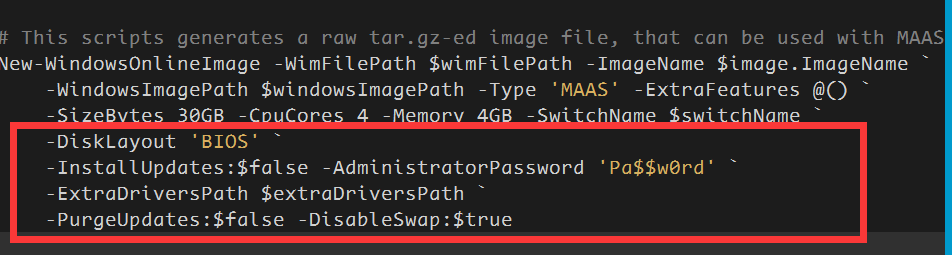
\includegraphics[width=\linewidth]{ps3.png}
  \caption{ps3}
  \label{fig:ps3}
\end{figure}

以管理员权限运行powershell,执行如下命令
\begin{code-block}{bash}
cd e:\windows-openstack-imaging-tools
cd Examples
.\create-windows-online-cloud-image.ps1
\end{code-block}

之后的过程基本就是全自动化,无需人工干预。成功之后,生成一个E:/hyper-v/windows.raw.tgz文件,
这个文件就是我们需要的ironic的windows镜像文件。如果制作过程中提示错误,可以重复执行。如果
制作过程中提示qemu-img出现错误,并且已经生成了一个E:/hyper-v/windows.raw.vhd或者
E:/hyper-v/windows.raw.vhdx文件,也可以认为镜像制作完毕,只是最后需要我们手工转换一下
转换vhd和vhdx文件的操作,最好切换到linux的环境下操作,操作如下:
\begin{code-block}{bash}
qemu-img convert -O raw windows.raw.vhdx /opt/windows.raw
\end{code-block}

生成的windows.raw就是我们最终需要的镜像文件,可以直接提供给ironic进行物理机的操作系统推送了。

cloud-init.conf的具体内容
\begin{code-block}{yaml}
users:
 - default
disable_root: 0
ssh_pwauth:   1
locale_configfile: /etc/sysconfig/i18n
mount_default_fields: [~, ~, 'auto', 'defaults,nofail', '0', '2']
resize_rootfs_tmp: /dev
ssh_deletekeys:   0
ssh_genkeytypes:  ~
syslog_fix_perms: ~
datasource:
  OpenStack:
    timeout: 5
    max_wait: 10
cloud_init_modules:
 - migrator
 - bootcmd
 - write-files
 - growpart
 - resizefs
 - update_etc_hosts
 - rsyslog
 - users-groups
 - ssh
 - runcmd
cloud_config_modules:
 - set-passwords
 - mounts
 - locale
 - yum-add-repo
 - package-update-upgrade-install
 - timezone: Asia/Shanghai
 - puppet
 - chef
 - salt-minion
 - mcollective
 - disable-ec2-metadata
cloud_final_modules:
 - rightscale_userdata
 - scripts-per-once
 - scripts-per-boot
 - scripts-per-instance
 - scripts-user
 - ssh-authkey-fingerprints
 - keys-to-console
 - phone-home
 - final-message: "Welcome to the Cloud World!"
system_info:
  default_user:
    name: root
    lock_passwd: false
    gecos: Cloud User
    groups: [wheel, adm, systemd-journal]
    sudo: ["ALL=(ALL) NOPASSWD:ALL"]
    shell: /bin/bash
  distro: rhel
  paths:
    cloud_dir: /var/lib/cloud
    templates_dir: /etc/cloud/templates
  ssh_svcname: sshd
# vim:syntax=yaml
\end{code-block}
